% =========================================================================
\documentclass[notes, aspectratio=1610]{beamer}
%\documentclass[aspectratio=1610]{beamer}

% ========================= Theme =========================================
\usetheme{Berkeley}
\usecolortheme{seahorse}

% ========================= Essential packages ============================
%\usepackage{hyperref}
%\hypersetup{
%    colorlinks = true,
%    linkcolor = blue,
%    citecolor = blue,
%    filecolor = blue,
%    urlcolor = blue
%}

% ========================= Frame notes systm ============================
%\usepackage{pgfpages}
%\setbeameroption{show notes on second screen}

% ========================= Plotting ======================================
\usepackage{calc}
\usepackage{tikz}
\usetikzlibrary{arrows,
                arrows.meta,
                calc,
		chains,
                quotes,
                positioning,
		shapes,
                shapes.geometric}
\usepackage{graphicx}
\usepackage{graphics}
\usepackage{pgfplots}
\pgfplotsset{width=7cm,compat=1.17}

%% ============================== Tabular =================================
\usepackage{booktabs}
\usepackage{tabularx,ragged2e}
\usepackage{array}
\usepackage{multirow}
\usepackage{siunitx}
  \sisetup{detect-all}
\usepackage{adjustbox}
\usepackage{rotating}
\usepackage{threeparttable}
\usepackage[justification=centering]{caption}
\usepackage{color, colortbl}

%% ============================== Text boxes ==============================
\usepackage[most]{tcolorbox}		

% ========================= Infor on authors ==============================
%\title[Visualization Design]%
%{Visualization Design}
\title{Geospatial Data Visualization}
\author{S.~Santoni\inst{1}\inst{2}}
\institute{
	\inst{1}%
	Bayes Business School
	\and
	\inst{2}%
	Soundcloud
	}
\date{MSc in Business Analytics, 2022/23}

% ============================ Colors =====================================
\definecolor{base_c}{rgb}{0.6,0,0}
\definecolor{comp_c}{rgb}{0.09803921568627451, 0.6901960784313725, 0.7529411764705882}
\definecolor{tri_1}{rgb}{0.09803921568627451, 0.7686274509803922, 0.19215686274509805}
\definecolor{tri_2}{rgb}{0.19215686274509805, 0.09803921568627451, 0.7686274509803922}

% ========================= TOC  ==========================================
\AtBeginSection[]
{
	\begin{frame}
		       \frametitle{Outline}
		       \tableofcontents[currentsection,currentsubsection]
	\end{frame}
}

% ========================= References ===================================
\usepackage[style=numeric,backend=biber]{biblatex}
\addbibresource{bibliography.bib}

% ========================= Document  ====================================
\begin{document}

\begin{frame}
	\titlepage
\end{frame}

\begin{frame}{Outline}
	\tableofcontents
\end{frame}

% ========================== Historical aspects ===========================
\section{The History of Geospatial Data Visualization}

\begin{frame}{Dr Snow's Study of Cholera Spread in 19\textsuperscript{th} 
	Century London}{}
	
	\centering 

	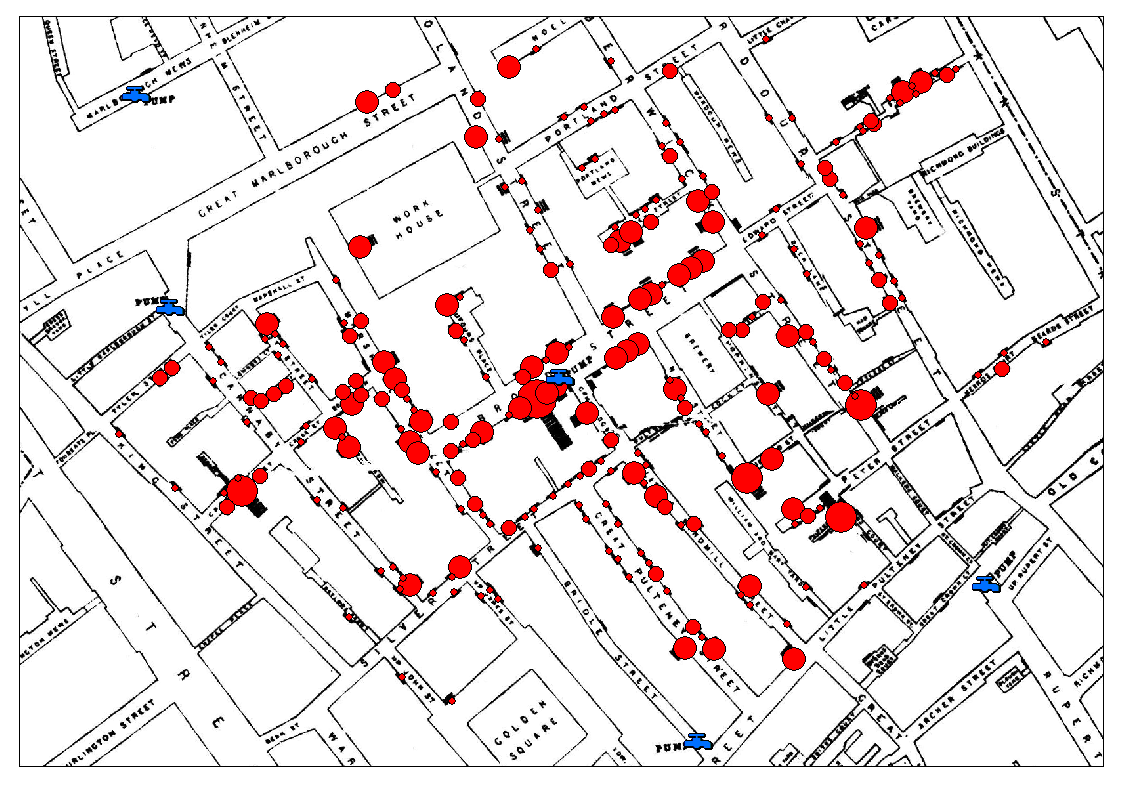
\includegraphics[width=0.75\textwidth]{images/SnowMap_Points.png}

	Go to the video: \url{https://www.youtube.com/watch?v=Pq32LB8j2K8}
\end{frame}

% ======================= Methodological aspects ===========================
\section{Methodological Aspects}

\begin{frame}{What Are the Methodological Roots of Geo-Spatial Analyses?}
	\begin{itemize}
		\item 
		Geographic Inforamtion Systems (GIS)
		\item 
		Remote sensoring
		\item 
		Elevation data
	\end{itemize}
\end{frame}

\begin{frame}{GIS}{}
	\begin{columns}
	\begin{column}{0.5\textwidth}
		\begin{itemize}
		\item 
		Computer mapping evolved with the computer itself in the 1960s
		\item 
		The term GIS began with the Canadian Department of Forestry 
		and Rural Development
			\begin{itemize}
				\item 
				Dr. Roger Tomlinson headed a team of 40 
				developers in an agreement with IBM to build the 
				Canada Geographic Information System (CGIS)
			        \item 
				The CGIS tracked the natural resources of Canada 
				and allowed the profiling of these features for further 
				analysis
			      	\item 
				The CGIS stored each type of land cover as a different 
				layer
			\end{itemize}
		\end{itemize}
	\end{column}
	\begin{column}{0.5\textwidth}
		\centering
		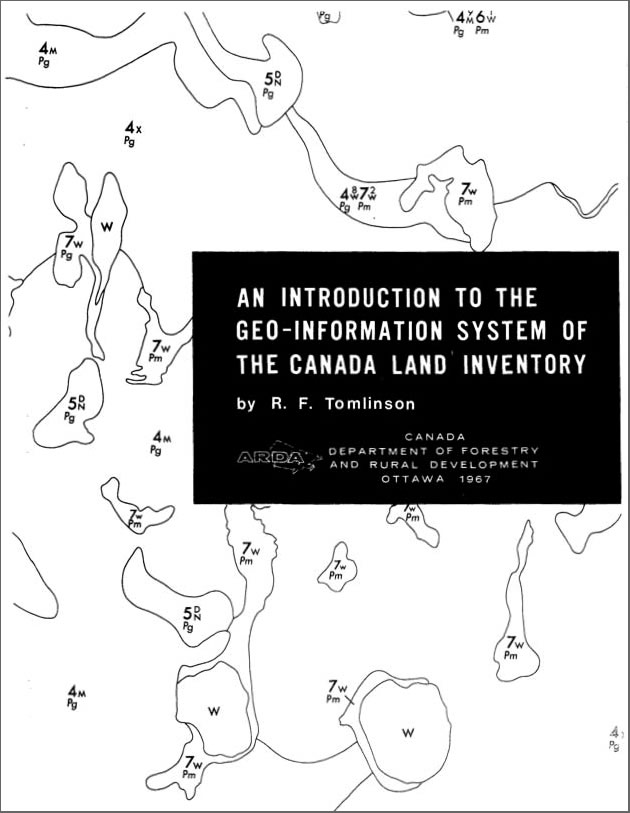
\includegraphics[width=0.8\textwidth]{images/canada_gis.jpeg}
	\end{column}
	\end{columns}
\end{frame}

\begin{frame}{An Example of GIS}{}
	\centering 

	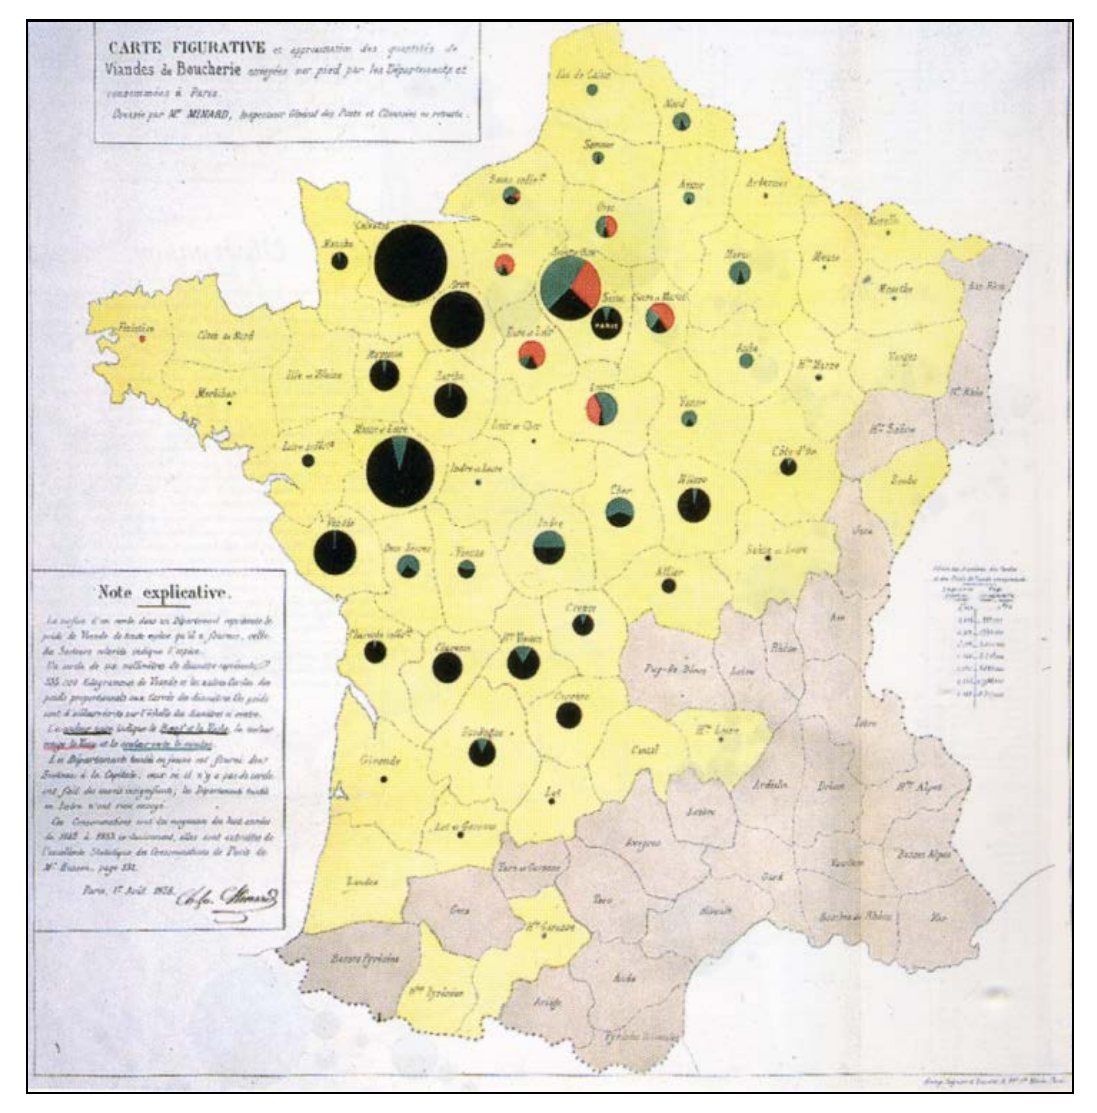
\includegraphics[width=0.5\textwidth]{images/example_of_gis.png}

	\small 

	Source: Minard (early 1900s)
\end{frame}

\begin{frame}{Remote Sensoring}{}
	\begin{columns}
		\begin{column}{0.5\textwidth}
		\begin{itemize}
			\item 
			\textbf{Remote sensing} is the collection of information about an 
			object without making physical contact with that object
			\item 
			In the context of geospatial analysis, the object is usually 
			the Earth
			\item 
			By extracting features from images, modern remote sensing 
			technologies have enabled GIS
		\end{itemize}
		\end{column}
		\begin{column}{0.5\textwidth}
		\centering
		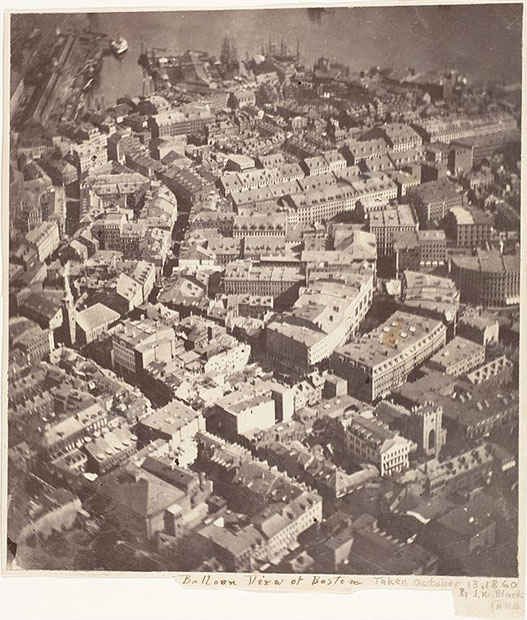
\includegraphics[width=0.8\textwidth]{images/56914f0d6cbe4.jpeg}
		\end{column}
	\end{columns}
\end{frame}

\begin{frame}{Elevation Data}{}
	\begin{columns}
		\begin{column}{0.5\textwidth}
		\begin{itemize}
			\item 
			A Digital Elevation Model (DEM) is a three-dimensional 
			representation of a planet's terrain (e.g., the Earth)
			\item 
			Before computers, representations of elevation data were 
			limited to topographic maps created through traditional land 
			surveys
			\item 
			Technology existed to create three-dimensional models from 
			stereoscopic images or physical models from materials such as 
			clay or wood
		\end{itemize}
		\end{column}
		\begin{column}{0.5\textwidth}
		\centering
		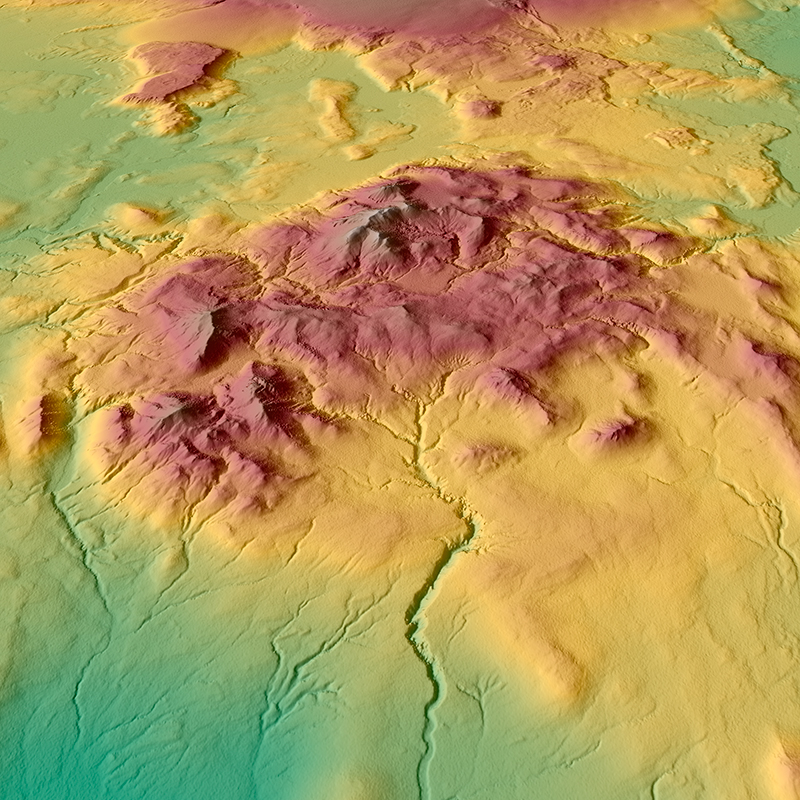
\includegraphics[width=0.8\textwidth]{images/worlddem_south_province_iceland_2012.jpg}
		\end{column}
	\end{columns}
\end{frame}

% ============== Geospatial data viz challenges ============================
\section{The Challenges of Geospatial Data Visualization}

\begin{frame}{Geographic Vs. Screen Coordinates}{}
    \begin{itemize}
    	\item Geographic data are stored in a coordinate system representing a 
    	grid overlaid on the Earth, which is \textcolor{blue}{three-dimensional}
	and \textcolor{purple}{round}
	\pause
    	\item Screen coordinates, also known as pixel coordinates, represent a 
    	grid of pixels on a \textcolor{blue}{two-dimensional} and \textcolor{purple}
	{flat} computer screen
	\pause
    	\item Mapping $x$ and $y$ world coordinates to pixel coordinates is fairly 
    	straightforward and involves a simple scaling algorithm
	\pause
    	\item However, if a $z$ coordinate exists, then a more complicated 
    	transform must be performed to map coordinates from three-dimensional 
    	space to a two-dimensional plane
    \end{itemize}
\end{frame}

\begin{frame}{Geographic Vs. Screen Coordinates}
	{How to build a stripped down version of a GIS}
	\begin{enumerate}
		\item Data model setup 
		\item Fix map size 
		\item Scaling the map 
		\item Sample GIS function 
		\item Render the map
	\end{enumerate}
\end{frame}

\begin{frame}{How to Build a Stripped Down Version of a GIS}
	{Step 1: data model setup}
	Let us set up the data for a sample USA state (Colorado) as a 
	list with name, polygon points, and population

	\centering

	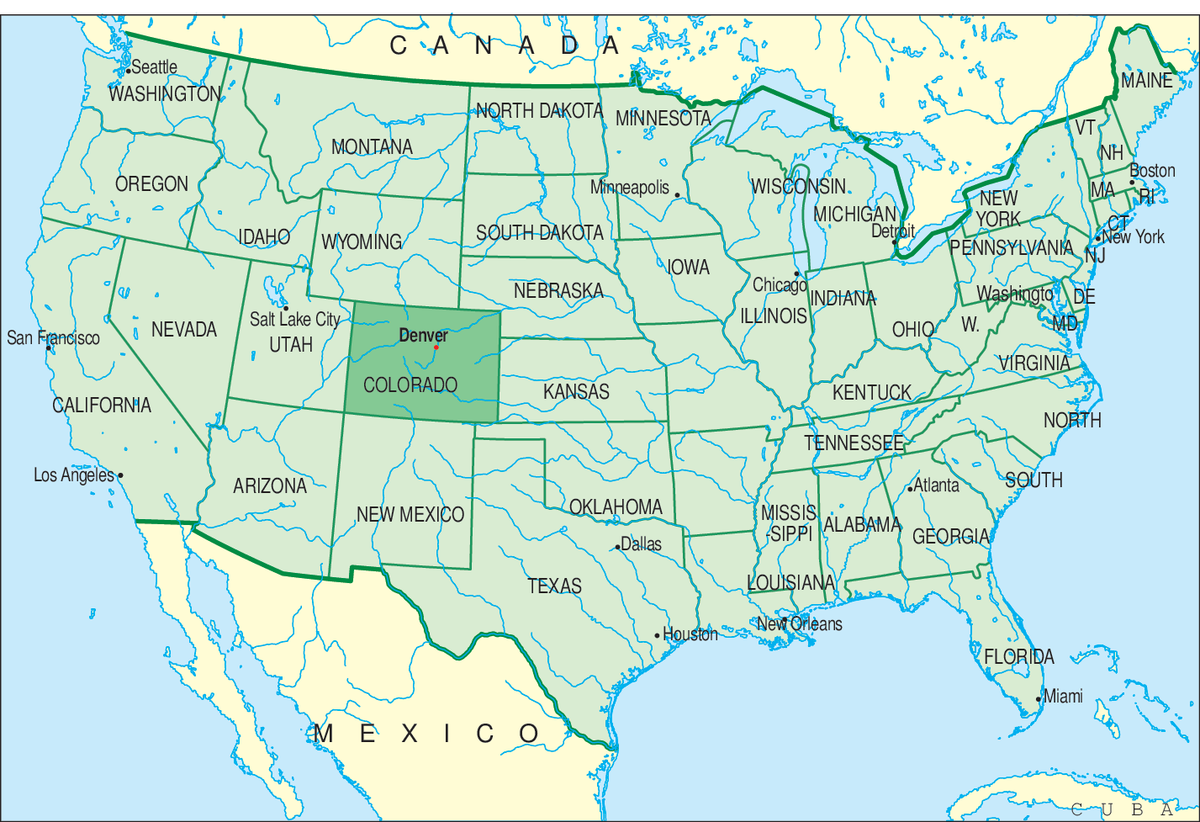
\includegraphics[width=0.6\textwidth]{images/colorado}
\end{frame}

\begin{frame}{How to Build a Stripped Down Version of a GIS}{Steps 2 - 5}
\centering
\Large
Let us move to Python!
\end{frame}

% ======================= Geospatial data viz modules ======================
\section{Python Modules for Geospatial Data Visualization}

\begin{frame}{The Python Geospatial Viz Ecosystem is VERY Rich!}{}
	\centering 
	\Large
	Please refer to the Jupyter Notebook file \texttt{python\_modules.ipynb}
\end{frame}

% =========================== Bibliography =================================
%\begin{frame}
%	\frametitle{References}
%	\printbibliography
%\end{frame}

% =========================== Close ========================================
\end{document}